\documentclass[notes]{beamer}          % print frame + notes
%\documentclass[notes=only]{beamer}     % only notes
%\documentclass{beamer}                 % only frames

\usecolortheme{beaver}

% Some commonly used packages
% (copied mainly from the Utrecht University theme: https://www.overleaf.com/project/5c900fa3bd9930036341116a)
\usepackage{ragged2e}  % `\justifying` text
\usepackage{booktabs}  % Tables
\usepackage{tabularx}
\usepackage{tikz}      % Diagrams
\usetikzlibrary{calc, shapes, backgrounds}
\usepackage{amsmath, amssymb, amsfonts, amsthm}
\usepackage{url}       % `\url`s
\usepackage{listings}  % Code listings
\usepackage{comment}
\usepackage{mathtools}
\usepackage{graphicx}
\usepackage{subfig}
\usepackage{bm}

% Mainly math commands
\newcommand{\vect}[1]{\bm{#1}}
\usepackage{amsfonts}% to get the \mathbb alphabet
\newcommand{\field}[1]{\mathbb{#1}}
\newcommand{\C}{\field{C}}
\newcommand{\R}{\field{R}}
\newcommand{\norm}[1]{\left\lVert#1\right\rVert}
\newcommand{\argmin}{\operatornamewithlimits{argmin}}
\providecommand{\abs}[1]{\lvert#1\rvert}
\providecommand{\norm}[1]{\lVert#1\rVert}

% A variable used to exclude slides from the lecture version
\newif\iffull
%\fullfalse
\fulltrue

% Bibliography
\usepackage[uniquename=init,giveninits=true,maxcitenames=1,style=authortitle-comp]{biblatex}
\bibliography{lectures/references}

%Information to be included in the title page:
\title{Course introduction 2019}
\author{Mitko Veta}
\institute{Eindhoven University of Technology

Department of Biomedical Engineering}
\date{2019}
 
 
 
\begin{document}
 
\frame{\titlepage}

\begin{frame}
\frametitle{Why machine learning?}
\begin{center}
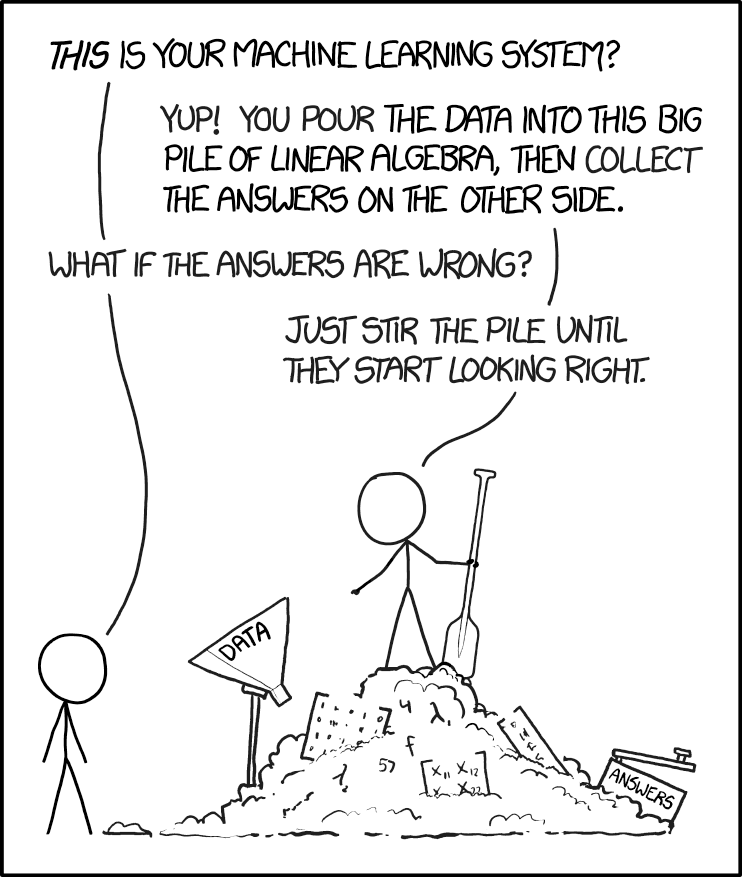
\includegraphics[height=7cm]{figures/intro/machine_learning.png}
\end{center}
{\tiny Figure source: xkcd.com}
\end{frame}

\begin{frame}
\frametitle{Historical perspective}
\begin{center}
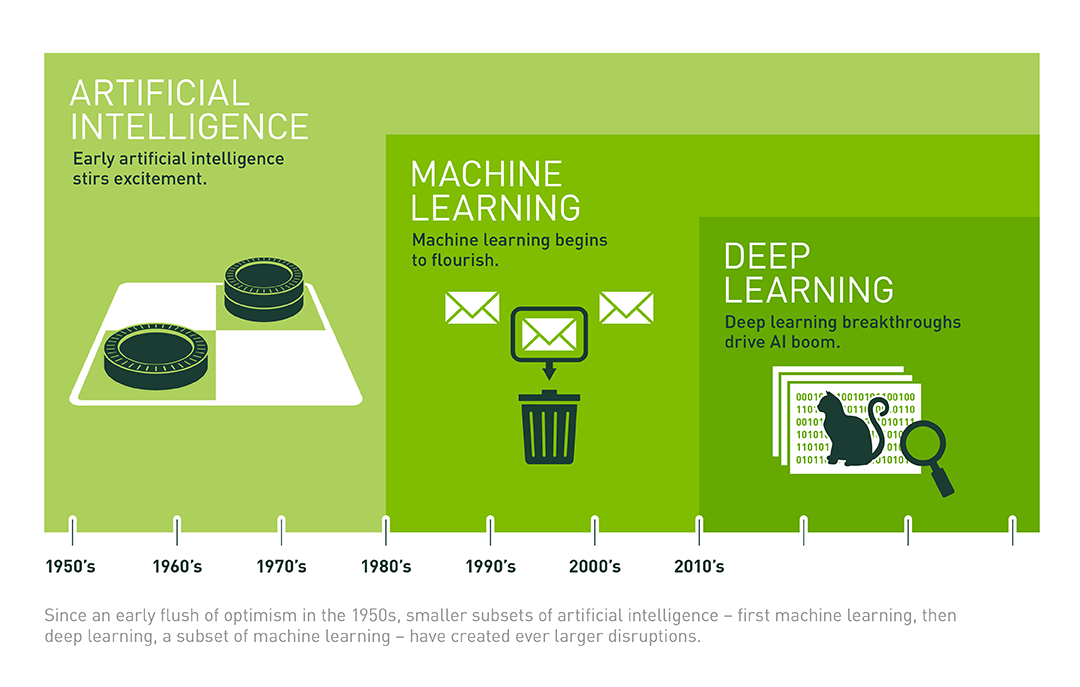
\includegraphics[height=7cm]{figures/intro/deep_learning.png}
\end{center}
{\tiny Figure source: nvidia.com}
\end{frame}

\begin{frame}{The course in a nutshell}
\begin{itemize}
    \item Seven topics
    \begin{itemize}
        \item Six lectures and practicals
        \item One self-study topic
    \end{itemize}
    \item{Assessment}
        \begin{itemize}
            \item 65\% written exam
            \item 25\% practicals
            \item 10\% presentations of self-study topic
            \item 0\% \textbf{mandatory} Python self-assessment quiz in the first week
        \end{itemize}
    \item GitHub repository used for material dissemination
    \item Canvas used for communication and submissions/grading
    \item Lectures every week (for the first six weeks of the quartile) on Wednesdays, time slots 1 and 2 
    \item Practicals immediately after the lectures, time slots 3 and 4
    
\end{itemize}
\end{frame}

\begin{frame}{Topics covered in the course}
\begin{itemize}
    \item Machine learning fundamentals I (Mitko Veta)
    \item Machine learning fundamentals II (Mitko Veta)
    \item Linear models (Federica Eduati)
    \item Deep learning I (Mitko Veta)
    \item Deep learning II (Jelmer Wolterink, UMCU/UvA)
    \item Support vector machines, random forests (Federica Eduati)
    \item Unsupervised machine learning (self study topic)
\end{itemize}
\end{frame}

\begin{frame}{Study materials}
\begin{itemize}
\item Main: lecture slides and practicals
\item Books
\begin{itemize}
    \item \cite{deeplearning}
    \item \cite{elements}
\end{itemize}
\item Specific chapters and additional material (such as papers) are referenced in the lecture slides
\end{itemize}
\end{frame}

\begin{frame}{Practicals}
\begin{itemize}
    \item Distributed as Python notebooks
    \item Deliverables
    \begin{itemize}
        \item Python functions and/or classes (.py files) that implement basic functionalities (e.g. a $k$-NN classifier)
        \item A \textbf{single} Python notebook that contains the experiments, visualization and answer to the questions and math problems.
    \end{itemize}
    \item The assessment rubric for the practicals can be found in the handouts for week 1
    \item Use of GitHub is highly recommended 
    \item The essential skills tutorial covers Python and git basics
\end{itemize}    
\end{frame}

\end{document}
